\section{Experiment Execution Procedure}
\label{sec:execution-procedure}

To ensure statistical reliability and eliminate operator and learning biases, the experimental execution follows a strictly automated and repeatable protocol across all 30 iterations ($N=30$) per scenario \cite{wohlin_2012}. Rather than relying on human operators navigating terminal prompts or graphical interfaces, both the baseline (Scenario~3) and experimental (Scenario~4) diagnostic workflows are executed autonomously by a deterministic Root Cause Analysis (RCA) engine \cite{wang_2024, barata_2026}. The execution procedure follows four sequential phases:

\begin{enumerate}
    \item \textbf{State Restoration and Warm-up:} Prior to each iteration, the cluster environment is restored to a validated, healthy baseline. The orchestrator removes any previously injected chaos resources and issues a \texttt{kubectl rollout status} check across the microservices namespace to confirm that all pods are 100\% available and healthy. A mandatory 20-second cooldown period is enforced to purge pending TCP connections, clear transient kernel queues, and stabilize CPU, memory, and network I/O to steady-state levels \cite{jain_1991, georges_2007}.
    
    \item \textbf{Load Generation:} The polyglot Astronomy Shop workload operates under steady-state traffic driven by its native \textit{loadgenerator} microservice. Synthetic user sessions actively traverse the inter-service graph (e.g., product catalog queries, cart mutations, and checkout sequences) prior to perturbation.
    
    \item \textbf{Blind Fault Injection ($T_0$):} Faults are injected programmatically via Chaos Mesh by applying a calibrated network delay ($2000\,\text{ms} \pm 100\,\text{ms}$) to target pods. To ensure experimental neutrality, a blind randomized injector selects the target microservice at runtime from the critical transaction path ($\text{Pool} = \{\texttt{payment}, \texttt{cart}, \texttt{shipping}, \texttt{currency}\}$). The exact RFC3339 timestamp of the Kubernetes API Server submission is recorded as the authoritative injection start time ($T_0$).
    
    \item \textbf{Algorithmic Diagnosis and Latency Extraction ($T_{\text{diag}}$):} Upon fault activation and an initial 10-second propagation window, the automated diagnostic engine initiates periodic polling (every $5\,\text{s}$) to isolate the injected root cause:
    \begin{itemize}
        \item \textbf{Vanilla Kubernetes (Scenario~3):} The engine interacts exclusively with native Kubernetes CLI endpoints, executing breadth-first log scraping constrained by temporal \texttt{--since-time} filters, regex exception matching, and periodic resource polling via the \texttt{metrics-server} API \cite{wang_2024}.
        \item \textbf{PANOPTES Architecture (Scenario~4):} The engine queries the unified telemetry backends, sampling upper percentile latencies ($p95/p99$) via Prometheus HTTP endpoints, querying Tempo for traces exhibiting anomalous duration, and traversing the call graph to isolate the root span \cite{barata_2026}.
    \end{itemize}
\end{enumerate}

The Mean Time to Diagnose ($MTTDiag$) for each iteration is recorded as the wall-clock execution latency between fault injection and algorithmic convergence:
\begin{equation}
    MTTDiag = T_{\text{diag}} - T_0
\end{equation}
If the diagnostic engine fails to converge on the ground-truth component or exceeds the operational ceiling of $300\,\text{s}$ ($5\,\text{min}$), the iteration is right-censored at $300\,\text{s}$ and flagged as an investigative failure ($Acc = 0$, $\text{censored} = \text{True}$).

\subsection{Automated Orchestration Lifecycle}
\label{subsec:automated-orchestration-lifecycle}

To guarantee experimental replicability and eliminate operator fatigue, observer bias, and clock desynchronization, the complete lifecycle across both experimental groups is governed by out-of-band automation scripts (\texttt{run-scenario3-trials.py} and \texttt{run-scenario4-trials.py}).

The orchestration pipeline executes an automated state machine for each experimental trial:
\begin{enumerate}
    \item \textbf{Cluster State Synchronization:} The orchestrator queries the Kubernetes API to guarantee that all microservices deployments have fully recovered from the preceding trial (\texttt{kubectl rollout status}), followed by the 20-second quiet period to purge transient network buffers and conntrack table entries.
    
    \item \textbf{Dynamic Fault Manifest Generation:} The orchestrator dynamically synthesizes and applies the Chaos Mesh manifest (\texttt{NetworkChaos}) targeting the blindly selected microservice and captures the RFC3339 timestamp ($T_0$).
    
    \item \textbf{Temporal Isolation and Active Polling:} Following a 10-second delay to allow traffic propagation, the RCA engine initiates polling. In the Vanilla baseline, queries to container logs enforce a strict temporal boundary (\texttt{--since-time=}$T_0$), preventing cross-trial contamination from historical log entries.

    \item \textbf{Ground-Truth Convergence and Data Persistence:} When the engine emits its diagnostic verdict, the timestamp is captured as $T_{\text{diag}}$, computing $MTTDiag$. If the diagnosed component matches the ground truth, accuracy is recorded as $Acc = 1$; otherwise, or upon reaching the 300-second ceiling, it is recorded as $Acc = 0$. The trial tuple ($\text{trial\_id}$, $\text{ground\_truth}$, $\text{diagnosed\_target}$, $T_0$, $MTTDiag$, $Acc$, $\text{censored}$) is written to persistent storage, and the chaos manifest is removed.
\end{enumerate}

\subsection{Testbed Commissioning and Telemetry Validation}
\label{subsec:testbed-commissioning}

Prior to the execution of the full $N=30$ trial batteries across the experimental groups, the testbed underwent systematic commissioning and functional validation. This stage verified that the deployment manifests, container runtimes, telemetry pipelines, and fault-injection hooks interact as specified in the architectural design.

\begin{figure}[htbp]
  \centering
  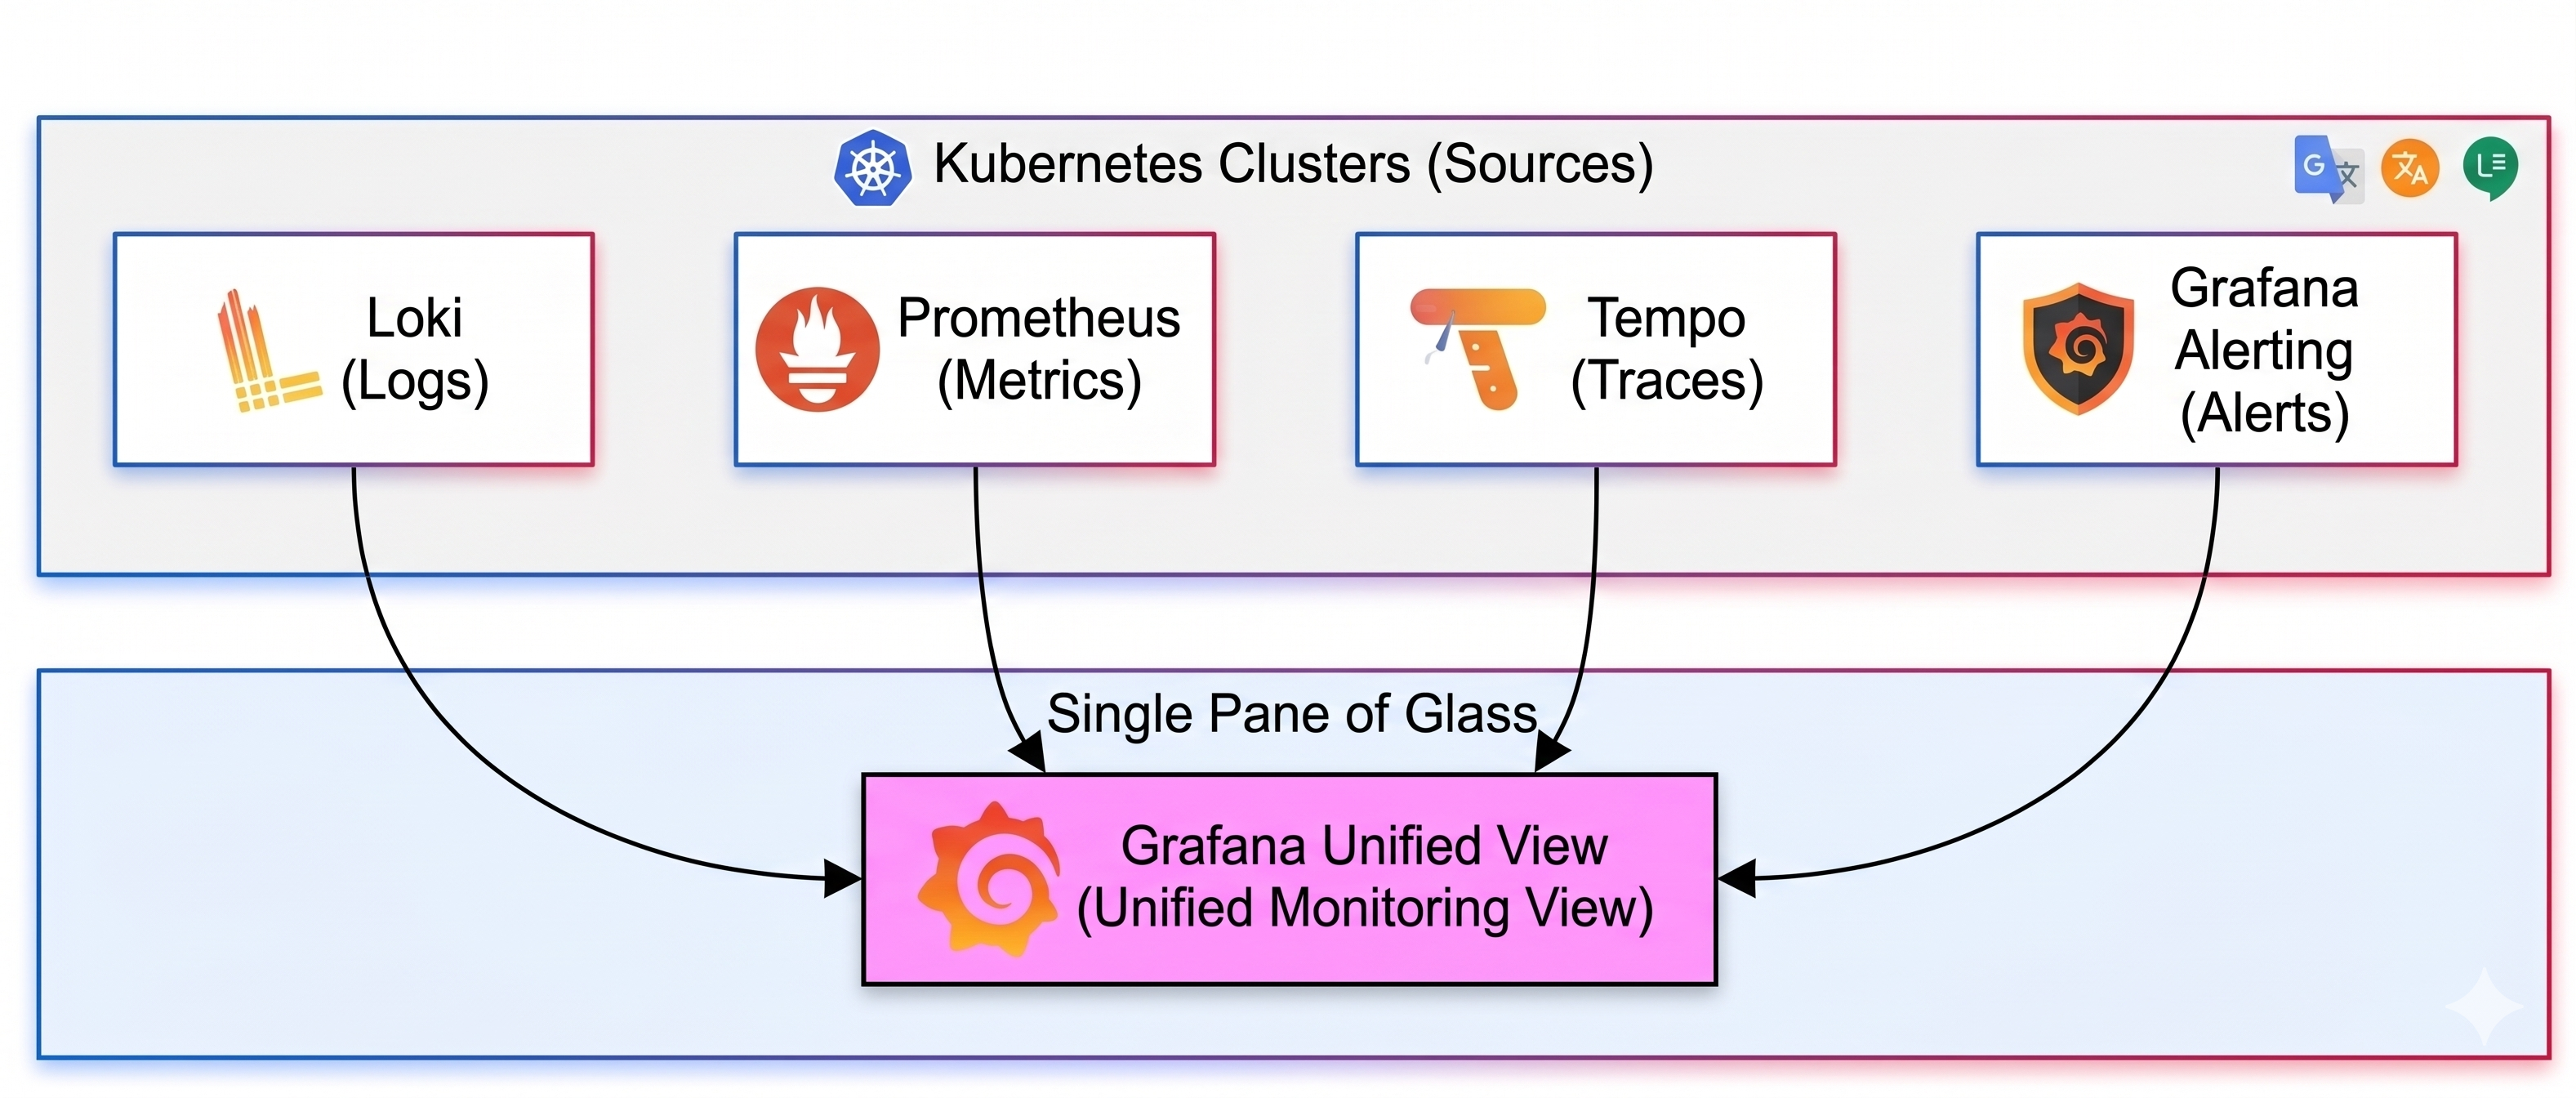
\includegraphics[width=0.9\textwidth]{images/experiment/grafana_preliminary.png}
  \caption{Single Pane of Glass dashboard validating unified telemetry ingestion in Grafana.}
  \label{fig:grafana_preliminary}
\end{figure}

Figure~\ref{fig:grafana_preliminary} demonstrates the operational ``Single Pane of Glass'' dashboard during steady-state workload execution. It validates that the OpenTelemetry collectors actively extract spans, runtime metrics, and container logs from the polyglot microservices, successfully streaming them to their respective storage backends: Prometheus, Grafana Loki, and Grafana Tempo. Furthermore, controlled perturbation trials confirmed that Chaos Mesh successfully manipulates the network namespaces of the target pods (applying netem delays) without destabilizing the underlying K3s control plane, establishing the safety and repeatability of the fault injection mechanism.

While the empirical evaluation of diagnostic latency ($MTTDiag$) is conducted autonomously via programmatic APIs to eliminate human operator bias, Grafana serves as the operational supervisory layer. It validates the underlying semantic binding implemented across the datasource configurations:
\begin{itemize}
    \item \textbf{Metrics to Traces via Exemplars:} The Prometheus datasource binds OpenTelemetry \texttt{traceID} values to latency histograms as exemplars. When an anomalous duration is recorded in the upper latency percentiles ($p95/p99$), the associated exemplar exposes the exact \texttt{traceID}, enabling immediate transition to the corresponding trace graph in Grafana Tempo without manual cross-system lookup.
    
    \item \textbf{Traces to Logs via Contextual Bindings:} The Tempo datasource integrates an automated \textit{Trace to Logs} mapping. For any anomalous span identified within a degraded execution path, the engine synthesizes a LogQL query for Loki. By scoping the search to the specific span timeframe, container namespace, and \texttt{traceID}, it bridges the gap between detecting inter-service latency inflation and inspecting the underlying execution context.
\end{itemize}

These integrated correlation pathways provide interactive root cause navigation within the Grafana interface for post-mortem analysis, while the deterministic RCA engine in Scenario~4 navigates this exact semantic topology programmatically via HTTP endpoints.